Для поиска кандидатов применялись данные, взятые из трёх каталогов точечных источников. За основу брался список всех источников, относящихся к рассматриваемой области, которые пронаблюдал телескоп GALEX.
Для этого списка проводилась кросс-идентификация с каталогами 2MASS и UCAC4 с целью получения данных о звёздных величинах в фильтрах инфракрасного и видимого диапазонов. 

%%%%%%%%%%%%%%%%%%%%%%%%%%%%%%%%%%%%%%%%%%%%%%%%%%%%%%%%%%%%%%%%%%%%%%%%%%%%%%%%%%%%%%%%

\section{GALEX}
GALEX (Galaxy Evolution Explorer) -- это ультрафиолетовый обзорный космический телескоп с полуметровым зеркалом, запущенный в 2003 году. Его целью является исследование эволюции звездообразования в галактиках от ранней вселенной до наших дней. Так как наблюдения в ультрафиолете недоступны с Земли, его каталог точечных источников является единственным источником данных в этом спектральном диапазоне.

\begin{figure}[ht]
\center{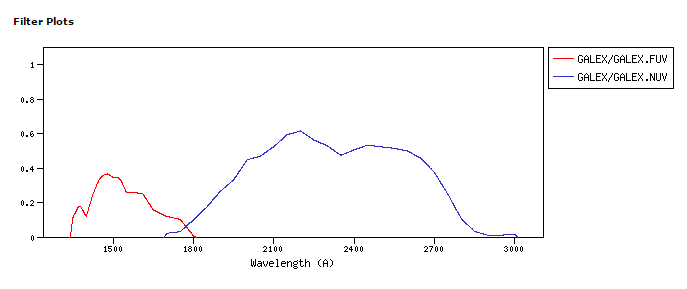
\includegraphics[width=1\linewidth]{filters.png}}
\hfill
\caption{Функции пропускания фильтров FUV и NUV космического телескопа GALEX}
\label{fig:filters}
\end{figure}

Обзор неба от GALEX состоит из круглых изображений радиусом 0.7 градусов и покрывает две трети небесной сферы. Наблюдения проводились в двух фильтрах: FUV(Far Ultraviolet), охватывающий диапазон 125-180 нм, и NUV(Near Ultraviolet) в диапазоне 170-300 нм с пространственным разрешением 4.3 и 5.3 угловых секунд соответственно.

Телескоп избегал наблюдений вблизи галактической плоскости и Магеллановых облаков, а также ярких звёзд, так как это могло привести к перегоранию чувствительных детекторов. Минимальная допустимая звёздная величина равна 9.5 и 8.9 для FUV и NUV соответственно. Максимальная звёздная величина составляет 22.3. Из-за высокой чувствительности телескопа в каталоге присутствует много ложных объектов, случайных шумов, которые были приняты за реальные источники. В дальнейшем эти паразитные источники отсеются при кросс-идентификации, не найдя соответствий в других спектральных диапазонах.

Так как интересующий нас участок неба находится близко к галактической плоскости, он не полностью покрыт наблюдениями, как это видно из рисунка \ref{fig:cover}. Для левой части туманности данных нет, а правая покрыта наблюдениями на 70\%.

\begin{figure}[ht]
\center{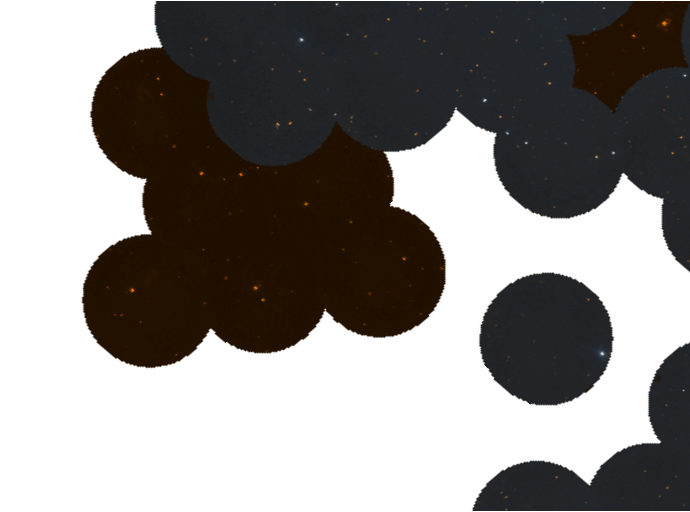
\includegraphics[width=0.6\linewidth]{cover.png}}
\hfill
\caption{Покрытие части изучаемой области наблюдениями телескопа GALEX}
\label{fig:cover}
\end{figure}

Для выбранной области нашлось 2968 источников, причём для некоторых из них отсутствовала звёздная величина в фильтре FUV. 

%%%%%%%%%%%%%%%%%%%%%%%%%%%%%%%%%%%%%%%%%%%%%%%%%%%%%%%%%%%%%%%%%%%%%%%%%%%%%%%%%%%%%%%%%%%%%%%%%

\section{Кросс-идентификация с 2MASS и UCAC4}
После получения исходного списка источников он был кросс-идентифицирован с каталогами 2MASS и UCAC4. То есть для каждого источника из списка мы искали соответствие в другом каталоге, основываясь на равенстве или близости их координат. Параметр кросс-корреляции взят равным 3 угловым секундам. Это максимальное расстояние между источниками из разных каталогов, при котором они будут считаться одним источником.

2MASS(Two Micron All-Sky Survey) -- это полный обзор всего неба на длинах волн около 2 микрон. Он содержит информацию о звёздных величинах в фильтрах J, H и Ks с длинами волн 1.25, 1.65 и 2.17 мкм соответственно.

Так как  этот обзор создавался с помощью больших наземных телескопов, пространственное разрешение здесь гораздо выше, чем у GALEX, и источники можно считать действительно точечными. Из-за низкой точности GALEX объекты в нём размазаны и эффективно имеют радиус около 2.2-2.7 угловых секунд. Поэтому при кросс-идентификации объект из GALEX считается совпавшим с объектом из 2MASS, если он попадает внутрь окружности с радиусом 3 угловых секунды.

Все источники из первоначального списка, не идентифицированные в каталоге 2MASS, должны быть сочтены ложными и откинуты.

Каталог UCAC4 содержит данные в фильтрах видимого диапазона: V и B фотометрической системы Джонсона, а также i и r фотометрической системы SDSS. Кроме того, из него мы берём информацию о собственных движениях звёзд. В него включены только звёзды. Их величины лежат в интервале от 8 до 16, ярче, чем в GALEX. Поэтому те объекты из списка, которые не нашли соответствия в UCAC4, не должны отбрасываться.

Инфракрасные звёздные величины необходимы нам для построения диаграмм цвет-цвет и формулирования критериев поиска звёзд типа Т Тельца. Величины в видимом диапазоне используются для иллюстрации на цветовых диаграммах и для дополнительного критерия. Также они нужны для оценки эффективных температур.

После кросс-идентификации список сократился до 726 объектов. 

\section{Используемые инструменты}
База данных миссии GALEX доступна посредством CasJobs. 

Данные всех используемых каталогов лежат в открытом доступе и могут быть получены с помощью сервиса Vizier. Также он может осуществлять кросс-идентификацию по координатам с заданным радиусом поиска в режиме онлайн. (The VizieR database of astronomical catalogues)
